%!TEX root = ../report.tex"
\section{Вопрос 56: Модель матрицы доступов Харрисона-Руззо-Ульмана (ХРУ). Теорема об алгоритмической неразрешимости задачи проверки безопасности произвольной системы ХРУ.}

\textbf{Модель ХРУ} реализует дискреционную политику управления доступом:
\begin{enumerate}
	\item Все сущности должны быть идентифициорованны
	\item Задана матрица доступов
	\item Субъект обладает правом доступа к сущности ТИТТК в заданной ячейке есть право доступа
\end{enumerate}

\begin{defs}[Модель ХРУ]
	\begin{enumerate}
		\item О -- множество объектов
		\item S -- множество субъектов
		\item R -- множество видов прав доступа субъектов к объектам (например read, write, own - владеть)
		\item M -- матрица доступов (строки представляют собой субъекты, столбцы - объекты)
	\end{enumerate}
\end{defs}

\begin{figure}[H]
	\centering
	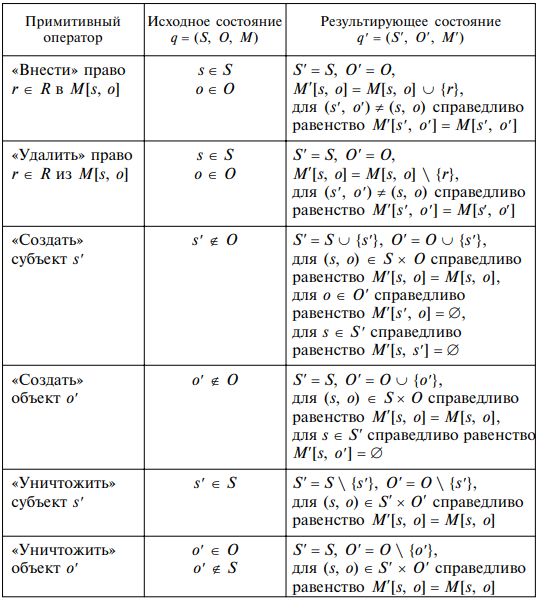
\includegraphics[width=0.5\linewidth]{img/1.png}
	\caption{Табличка}
\end{figure}

\begin{defs}[Утечка права]
	Будем считать, что в состоянии $q$ системы ХРУ возможна утечка права доступа $r \in R$ в результате выполнения команды С$\myvect{1}{n}$ в случае,
	когда при переходе системы $q \vdash_{c(x_1, \ldots, x_k)} q^{\shtrih}$ выполняется примитивный оператор, вносящий право доступа $r$ в ячейку матрицы доступов $M$, до этого $r$
	не содержащую.
\end{defs}

\begin{defs}[Безопасное начальное состояние]
	Начальное состояние $q_0$ системы ХРУ называется безопасным относительно некоторого права доступа $r \in R$ в случае, когда невозможен переход
	системы в такое состояние $q$, в котором возможна утечка права $r$.
\end{defs}

\begin{defs}[монооперационная система ХРУ]
	Система ХРУ называется монооперационной, когда каждая команда системы содержит один примитивный оператор.
\end{defs}

\begin{proofs}
	$\exists$ алгоритм, проверяющий является ли начальное состояние произвольной монооперационной системы ХРУ безопасным относительно некоторого
	права доступа $r \in R$.
\end{proofs}

\begin{proofs}[Об алгоритмической неразрешимости]
	Задача проверки безопасности произвольных систем ХРУ алгоритмически неразрешима.
	\begin{dokvo}
		Из теории машины Тьюринга: не существует алгоритма проверки для произвольной машины Тьюринга (МТ) и произвольного начального слова остановится ли МТ в конечном состоянии или нет.

		Представим все элементы и команды МТ в виде элементов и команд системы ХРУ.

		\textbf{МТ:}

		$ A = \{ \alpha_0, \ldots, \alpha_m \} $ -- внешний авлфавит, $ \alpha_0 = \wedge $ -- пустой символ.

		$ Q = \{ q_0, \ldots, q_k \} $ -- внутренний алфавит, $q_1$ -- начальное состояние, $q_0$ -- конечное.

		$ D = \{ r, l, e \} $ -- множество действий (вправо, влево, на месте).

		$ C: Q \times A \to Q \times A \times D $ -- функция, задающая команды МТ.

		Пусть МТ выполнила некоторое количество шагов. Пусть считывающая головка указывает на ячейку $ i \in \{ 1, \ldots , n \} $. $ (\alpha_{s_{1}}, \ldots, \alpha_{s_{n}}) $ -- заполненные ленты.

		$ R = Q \cup A \cup \{own, left, right \} $

		$ q_{ij} \in M[s_i, s_i] $ -- считывающая головка указывает на ячейку с номером $i$.

		$left \in M[s_1, s_1]$ -- признак крайней левой позиции

		$right \in M[s_n, s_n]$ -- признак крайней правой позиции

		Т.о. построим матрицу доступов:

		\begin{figure}[H]
			\centering
			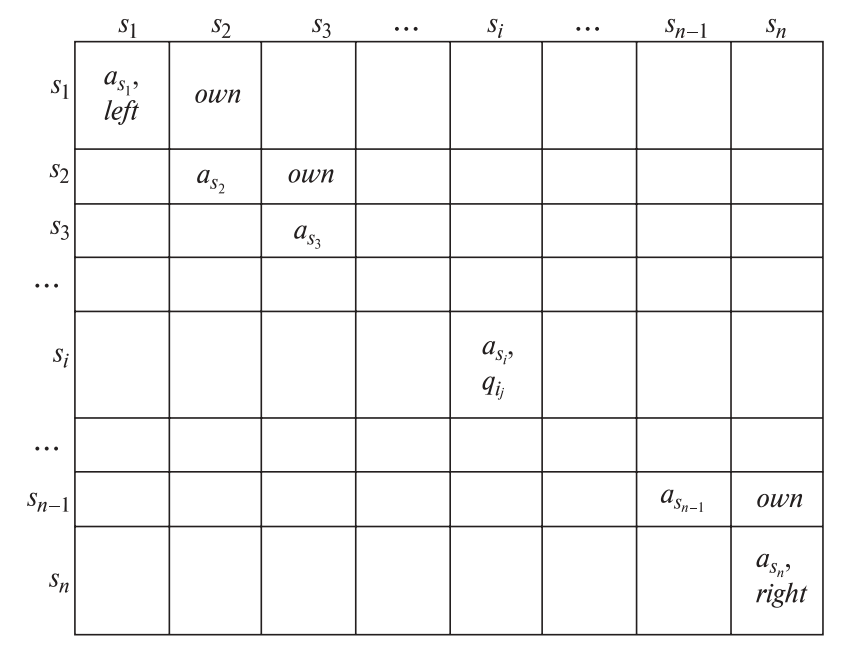
\includegraphics[width=0.5\linewidth]{img/2.png}
			\caption{Матрица доступов}
		\end{figure}

		Построим гомоморфизм машины Тьюринга в систему ХРУ. Зададим каждой команде МТ команду ХРУ:

		Если $d = e$, то

		$command E_{q_{i_{j}}a_{i_{t}}q_{i_{j^{\shtrih}}}a_{i_{t^{\shtrih}}}}(s)$

		$if (q_{i_{j}} \in M[s,s]) and (a_{i_{t}} \in M[s,s]) then $

		\kav{удалить} право $q_{i_{j}}$ из $M[s,s]$

		\kav{удалить} право $a_{i_{t}}$ из $M[s,s]$

		\kav{внести} право $q_{i_{j^{\shtrih}}}$ в $M[s,s]$

		\kav{внести} право $a_{i_{t^{\shtrih}}}$ в $M[s,s]$

		$endif$

		$end$

		Если $d = r$, то 2 случая (для крайней правой позиции и для другой произвольной)

		$command R1_{q_{i_{j}}a_{i_{t}}q_{i_{j^{\shtrih}}}a_{i_{t^{\shtrih}}}}(s, s^{\shtrih})$

		$if (q_{i_{j}} \in M[s,s]) and (a_{i_{t}} \in M[s,s])and (own \in M[s,s^{\shtrih}]) then $

		\kav{удалить} право $q_{i_{j}}$ из $M[s,s]$

		\kav{удалить} право $a_{i_{t}}$ из $M[s,s]$

		\kav{внести} право $a_{i_{t^{\shtrih}}}$ в $M[s,s]$

		\kav{внести} право $q_{i_{j^{\shtrih}}}$ в $M[s^{\shtrih},s^{\shtrih}]$

		$endif$

		$end$

		$command R2_{q_{i_{j}}a_{i_{t}}q_{i_{j^{\shtrih}}}a_{i_{t^{\shtrih}}}}(s, s^{\shtrih})$

		$if (q_{i_{j}} \in M[s,s]) and (a_{i_{t}} \in M[s,s])and (right \in M[s,s]) then $

		\kav{удалить} право $q_{i_{j}}$ из $M[s,s]$

		\kav{удалить} право $a_{i_{t}}$ из $M[s,s]$

		\kav{удалить} право $right$ из $M[s,s]$

		\kav{внести} право $a_{i_{t^{\shtrih}}}$ в $M[s,s]$

		\kav{создать} субъект $s^{\shtrih}$

		\kav{внести} право $own$ в $M[s,s^{\shtrih}]$

		\kav{внести} право $a_0$ в $M[s^{\shtrih},s^{\shtrih}]$

		\kav{внести} право $q_{i_{j^{\shtrih}}}$ в $M[s^{\shtrih},s^{\shtrih}]$

		\kav{внести} право $right$ в $M[s^{\shtrih},s^{\shtrih}]$

		$endif$

		$end$

		Аналогично для $d = l$. Из алгоритмической неразрешимости проверки, остановится ли МТ в своем конечном состоянии или нет следует
		алгоритмическая неразрешимость задачи проверки безопасности системы ХРУ.
	\end{dokvo}
\end{proofs}
\newpage
